\section{LLMs for Crop Science}
{{\footnotesize
\begin{description}[labelwidth=5em, labelsep=1em, leftmargin=*, align=left, itemsep=0.3em, parsep=0em]
  \item[date:] 2024-12-13
  \item[version:] TODO
  \item[last\_updated:] 2024-12
  \item[expired:] unknown
  \item[valid:] yes
  \item[valid\_date:] TODO
  \item[url:] \href{https://neurips.cc/virtual/2024/poster/97570}{https://neurips.cc/virtual/2024/poster/97570}
  \item[doi:] TODO
  \item[domain:] Agricultural Science; NLP
  \item[focus:] Evaluating LLMs on crop trait QA and textual inference tasks with domain-specific prompts
  \item[keywords:]
    - crop science
    - prompt engineering
    - domain adaptation
    - question answering
  \item[summary:] Establishes a benchmark of 3,500 expert-annotated prompts and QA pairs covering crop traits, growth stages, and environmental interactions. Tests GPT-style LLMs on accuracy and domain reasoning using in-context, chain-of-thought, and retrieval-augmented prompts.

  \item[licensing:] TODO
  \item[task\_types:]
    - Question Answering
    - Inference
  \item[ai\_capability\_measured:]
    - Scientific knowledge
    - crop reasoning
  \item[metrics:]
    - Accuracy
    - F1 score
  \item[models:]
    - GPT-4
    - LLaMA-2-13B
    - T5-XXL
  \item[ml\_motif:]
    - NLP
  \item[type:] Dataset
  \item[ml\_task:]
    - QA, inference
  \item[solutions:] TODO
  \item[notes:] Includes examples with retrieval-augmented and chain-of-thought prompt templates; supports few-shot adaptation.

  \item[contact.name:] Deepak Patel
  \item[contact.email:] unknown
  \item[results.links.name:] ChatGPT LLM
  \item[fair.reproducible:] Yes
  \item[fair.benchmark\_ready:] Yes
  \item[ratings.software.rating:] 0
  \item[ratings.software.reason:] Not analyzed.

  \item[ratings.specification.rating:] 9.0
  \item[ratings.specification.reason:] The task of ML correction to DFT energy predictions is well-specified.

  \item[ratings.dataset.rating:] 9.0
  \item[ratings.dataset.reason:] 10 public reaction datasets with DFT and CC references; well-documented.

  \item[ratings.metrics.rating:] 8.0
  \item[ratings.metrics.reason:] Uses MAE and ranking accuracy, suitable for this task.

  \item[ratings.reference\_solution.rating:] 8.0
  \item[ratings.reference\_solution.reason:] Includes both Delta\textasciicircum{}2 and KRR baselines.

  \item[ratings.documentation.rating:] 9.0
  \item[ratings.documentation.reason:] Public benchmarks and clear reproducibility via datasets and model code.

  \item[id:] llms\_for\_crop\_science
  \item[Citations:] \cite{shen2024exploringuserretrievalintegration}
  \item[Ratings:]
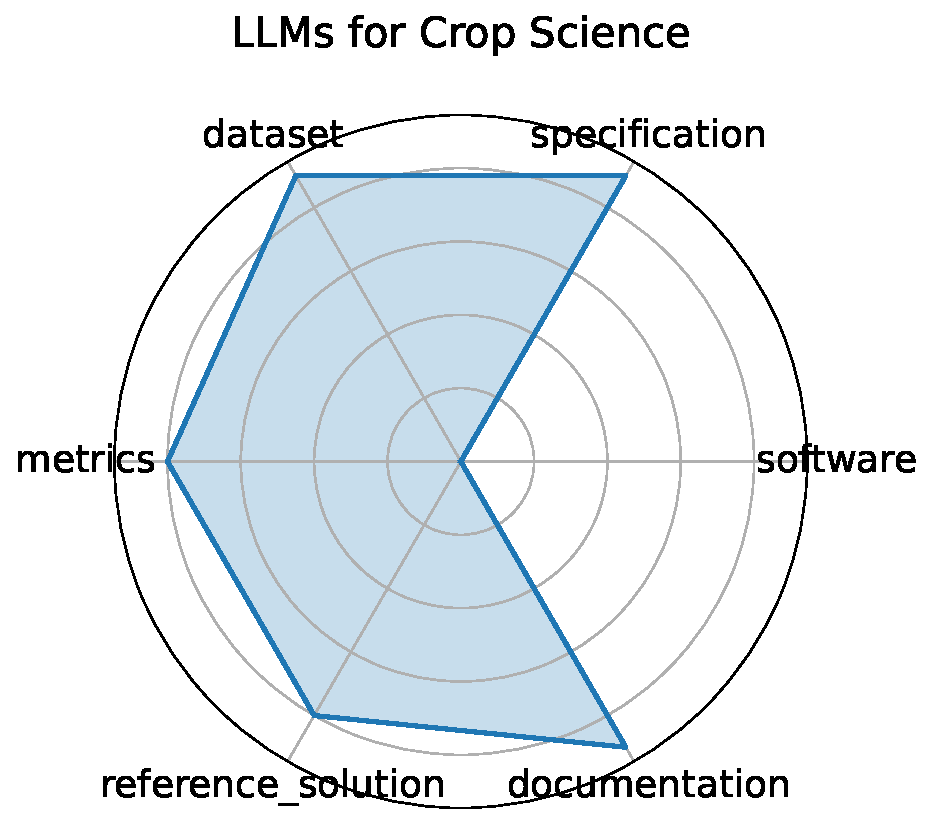
\includegraphics[width=0.2\textwidth]{llms_for_crop_science_radar.pdf}
\end{description}
}}
\clearpage